\section{Configuration}
\label{sec:config}
This section will highlight some of the configurations of Germinate 3. The configurations are stored in the file \texttt{\instanceStuff/<project.name>/config.properties}.

Currently the following settings are available:

\begin{lstlisting}[style=Properties]
Germinate.Database.Username=<username for the database>
Germinate.Database.Password=<password for the database

Germinate.Database.Server=<server of the germinate database>
Germinate.Database.Name=<name of the germinate database>
Germinate.Database.UsePort=<use a port for the connection?>
Germinate.Database.Port=<port for database connection>

Gatekeeper.URL=<base url of gatekeeper>
Gatekeeper.Database.Server=<server of the gatekeeper database>
Gatekeeper.Database.Name=<name of the gatekeeper database>
Gatekeeper.Database.UsePort=<use a port for the connection?>
Gatekeeper.Database.Port=<port for database connection>

Gatekeeper.BCrypt.Rounds=<number of rounds for the bcrypt hashing algorithm>
Gatekeeper.Registration.Enabled=<allow user registration?>
Gatekeeper.Registration.Needs.Approval=<user registration needs manual approval?>

Germinate.UseAuthentication=<users have to log in to see data?>
Germinate.CookieLifespanMinutes=<the lifespan of cookies in minutes>
Germinate.Debug=<enable to see sql queries run on the server>
Germinate.KeepTemporaryFileForHours=<how long should temporary files be kept?>
Germinate.UploadSizeLimitMB=<file size limit of uploads in MB>
Germinate.AvailablePages=<list of comma separated pages that are available for this instance of germinate>

Germinate.AccessionDisplayColumn=<the germinatebase column used for display purposes>
Germinate.BaseSearchColumn=<the germinatebase column used for the search and groups widget>
Germinate.CollectingsiteTreemapColumn=<the collecting sites column to group by for the treemap>
Germinate.ShowHomeOnLogin=<show the content of the home page on the login page as well?>

Germinate.Server.Logging.Enabled=<should exceptions be logged on the server?>

Germinate.IsUnderMaintenance=<is the server under maintenance?>

Germinate.IsReadOnly=<is the database in read-only mode?>

Germinate.ExternalDataFolder=<optional external data directory outside tomcat>

Germinate.HideIdColumns=<should internal id columns be hidden from tables?>

Germinate.Gallery.Images.Per.Page=<determines the number of images per page>

GoogleAnalytics.Enabled=<should google analytics be enabled?>
GoogleAnalytics.TrackingId=<the google analytics tracking id>

GoogleMaps.Api.Key=<the google maps api key to use>

CookieNotifier.Enabled=<should the cookie notifier for EU cookie law be enabled?>

Germinate.Template.CustomMenu=<the custom menu structure in XML format>

Germinate.Template.HighlightColor=<main color of all highlights on the interface>
Germinate.Template.CategoricalColors=<colors used for some of the charts>
Germinate.Template.Social.ShowFacebook=<show facebook share button?>
Germinate.Template.Social.ShowTwitter=<show twitter share button?>
Germinate.Template.Social.ShowGooglePlus=<show google+ share button?>
Germinate.Template.UseToggleSwitches=<show toggle switches?>
Germinate.Template.Show.Search=<show search in main menu?>
Germinate.Template.Logo.Contains.Link=<does the svg logo contain links?>
Germinate.Template.Show.Parallax.Banner=<show parallax image banner?>

Germinate.Template.EmailAddress=<contact email email address>

Germinate.Template.Title=<title of the germinate instance>
Germinate.Template.DatabaseName=<name of the germinate instance>
Germinate.Template.TwitterLink=<twitter link>
Germinate.Template.Copyright=<copyright information>

Path.Java=<path to the java installation>
Path.R=<path to the r installation>
\end{lstlisting}
\noindent
All items starting with \texttt{Germinate.Database} have already been discussed in Section \ref{sec:germinate-config}. Items starting with \texttt{Gatekeeper.Database} can be configured analogously.

We will now explain the meaning and possible settings of all the items. Non-optional properties are marked with "$\circ$" whereas "$*$" marks properties that are non-optional if you want to use the associated functionality. Unmarked properties either have a default value shown in \textbf{bold} or aren't crucial for Germinate to work properly.

\label{sec:config-properties}
\begin{description}
	\item[\texttt{Germinate.Database.Username}\nonoptional] \floatright{[String]}\\The MySQL username used for the Germinate 3 database.
	\item[\texttt{Germinate.Database.Password}\nonoptional] \floatright{[String]}\\The MySQL password associated with the username.
	\item[\texttt{Germinate.Database.Server}\nonoptional] \floatright{[String]}\\The server MySQL is running on.
	\item[\texttt{Germinate.Database.Name}\nonoptional] \floatright{[String]}\\The name of the Germinate 3 database.
	\item[\texttt{Germinate.Database.UsePort}] \floatright{[true \pipe \textbf{false}]}\\Set to \texttt{true} if a (non-standard) port should be used to connect to the database.
	\item[\texttt{Germinate.Database.Port}\nonoptionalif] \floatright{[$x\in\{0,\dots,49151\}$]}\\The actual port number.
	\item[\texttt{Gatekeeper.URL}\nonoptionalif] \floatright{[URL]}\\The URL of Germinate Gatekeeper. This is required if the registration feature is enabled. Refer to property \texttt{Germinate.Registration.Enabled} and Section \ref{sec:registration}.
	\item[\texttt{Gatekeeper.Database.Server}\nonoptionalif] \floatright{[String]}\\The server MySQL is running on.
	\item[\texttt{Gatekeeper.Database.Name}\nonoptionalif] \floatright{[String]}\\The name of the Germinate Gatekeeper database.
	\item[\texttt{Gatekeeper.Database.UsePort}] \floatright{[true \pipe \textbf{false}]}\\Set to \texttt{true} if a (non-standard) port should be used to connect to the database.
	\item[\texttt{Gatekeeper.Database.Port}\nonoptionalif] \floatright{[$x\in\{0,\dots,49151\}$]}\\The actual port number.
    \item[\texttt{Gatekeeper.BCrypt.Rounds}] \floatright{[$x\in \{4, \dots, \textbf{10}, \dots, 31\}$]}\\Gatekeeper uses BCrypt to hash passwords. The number of rounds determines how long the hashing will take. A larger number will make it harder to use brute-force to find the password, but at the same time it will influence how long users will have to wait for their password to be verified. The default is a value of $10$ which results in $2^{10}$ rounds. Increasing this to $11$ will \textbf{double the runtime} to $2^{11}$.
    \item[\texttt{Gatekeeper.Registration.Enabled}] \floatright{[true \pipe \textbf{false}]}\\Germinate and Gatekeeper support user registration. If this property is set to \texttt{true}, users will be able to register for access to your instance of Germinate. The registration will be accessible from the login page. See Section \ref{sec:registration} for more details.
    \item[\texttt{Gatekeeper.Registration.Needs.Approval}] \floatright{[\textbf{true} \pipe false]}\\If registration is enabled, there are two ways how users are approved for access to Germinate. If this property is set to \texttt{false}, users will automatically be approved and can start using Germinate right away. If this is not what you want, set this to \texttt{false} which will require you to approve requests manually through the Gatekeeper interface. Users will be notified with your decision via mail.
    \item[\texttt{Germinate.UseAuthentication}] \floatright{[true \pipe \textbf{false}]}\\If set to \texttt{true}, the user will have to log in using the credentials stored in Germinate Gatekeeper, otherwise no login procedure is required.
    \item[\texttt{Germinate.CookieLifespanMinutes}] \floatright{[$x\in\mathbb N^+$; default: \textbf{1440}]}\\The lifespan of all cookies given in minutes.
    \item[\texttt{Germinate.Debug}] \floatright{[true \pipe \textbf{false}]}\\Set to \texttt{true} if you want to see the SQL queries that are run against the database on each page. This is very handy when debugging or searching for errors. However, this should \textbf{never} \label{key}be used in production use, since it exposes the database internals.
    \item[\texttt{Germinate.KeepTemporaryFileForHours}] \floatright{[$x\in\mathbb N^+$; default: \textbf{24}]}\\The amount of hours temporary files should be kept for. Temporary files are generated whenever the user wants to download parts of the database. They are kept locally at least for the given amount of hours and after this amount of time they will be deleted the next time a user requests any temporary file.
    \item[\texttt{Germinate.UploadSizeLimitMB}] \floatright{[Float; default \textbf{0.5}]}\\The file size limit of uploads in MB.
    \item[\texttt{GoogleAnalytics.Enabled}] \floatright{[true \pipe \textbf{false}]}\\Germinate supports Google Analytics. Page navigation as well as user interactions will be tracked if this property is set to \texttt{true}.
    \item[\texttt{GoogleAnalytics.TrackingId}\nonoptionalif] \floatright{[String]}\\ The tracking id provided by Google Analytics.
    \item[\texttt{GoogleMaps.Api.Key}\nonoptionalif] \floatright{[String]}\\ The Google Maps API key. Starting from mid-2016 Google Maps requires websites to use an API key when using Google Maps. The key is free and can be acquired from this website:
    \begin{center}
    	\url{https://developers.google.com/maps/documentation/javascript/get-api-key}
    \end{center}
    \noindent
    \item[\texttt{CookieNotifier.Enabled}] \floatright{[true \pipe \textbf{false}]}\\ In accordance with the EU Cookie Law \cite{CookieLaw} we provide a notify banner at the bottom of the page that informs users that we use cookies. Set this to \texttt{false} to disable this banner.
    \item[\texttt{Germinate.AvailablePages}\nonoptional] \floatright{[CSV]}\\Not all pages are useful for all instances of Germinate. List the names of those pages that should be available for this instance in a comma-separated fashion, \eg \texttt{climate, megaEnvironments, gallery}.
    \item[\texttt{Germinate.AccessionDisplayColumn}] \floatright{[String; default: \textbf{name}]}\\Whenever accessions are displayed in charts, we need to show an identifier or a name of the accession. We allow the user to define which of the germinatebase table columns they want to use for this purpose.
    \item[\texttt{Germinate.BaseSearchColumn}] \floatright{[String; default: \textbf{name}]}\\On many parts of the page, the user is able to search for accessions based on a given column of the germinatebase table (\eg \texttt{name}, \texttt{number}, etc.). Specify this column name here to search in this column.
    \item[\texttt{Germinate.CollectingsiteTreemapColumn}] \floatright{[String; default: \textbf{country\textunderscore name}]}\\The column used to group the collecting sites for the treemap (\eg \texttt{region}, \texttt{country\_name}, etc.).
    \item[\texttt{Germinate.ShowHomeOnLogin}] \floatright{[true \pipe \textbf{false}]}\\If set to \texttt{true}, the login page will show the content of the home page as well. If set to \texttt{false}, the login page will only contain the text fields for the username and password.
    \item[\texttt{Germinate.Server.Logging.Enabled}] \floatright{[true \pipe \textbf{false}]}\\If set to \texttt{true}, exceptions will be logged on the server side. Otherwise, they will only be forwarded to the client and the client decides what to do with them.
    \item[\texttt{Germinate.IsUnderMaintenance}] \floatright{[true \pipe \textbf{false}]}\\If set to \texttt{true}, the web interface will be completely disabled, just showing a notification that the system is under maintenance.
    \item[\texttt{Germinate.IsReadOnly}] \floatright{[true \pipe \textbf{false}]}\\If set to \texttt{true}, the web interface will not allow the user to perform changes to the database, i.e., the generation/modification of user-created content will be disabled.
    \item[\texttt{Germinate.ExternalDataFolder}\nonoptionalif] \floatright{[Path]}\\If this property is set, Germinate will use the given path to look for files like images, data files and external applications. If the property is not set, Germinate will use the internal folders. This option can be useful if your data is huge and you don't want to include it in the generated war file, but rather want to store it in a different location on the server. Make sure that Germinate has read and write access to this folder.
    \item[\texttt{Germinate.HideIdColumns}] \floatright{[true \pipe \textbf{false}]}\\
    If set to \texttt{true}, the internal id column will be hidden from all tables.
    \item[\texttt{Germinate.Gallery.Images.Per.Page}] \floatright{[$x\in\mathbb N^+$; default: 16]}\\This setting determines how many images are shown per page on the gallery page.
    \item[\texttt{Germinate.Gallery.Make.Thumbnails.Square}] \floatright{[true \pipe \textbf{false}]}\\If set to \texttt{true}, the automatically generated thumbnails of images will be square to keep a uniform look across all thumbnails. The default is \texttt{false} to keep it consistent with previous versions.
    \item[\texttt{Germinate.Template.CustomMenu}] \floatright{[XML]}\\This allows you to customize the main menu of Germinate. Please consult Section \ref{sec:menu} for more details and an example.
    \item[\texttt{Germinate.Template.HighlightColor}] \floatright{[HEX; default: \textbf{\coloredtext{00ACEF}}]}\\The color used for all highlights on the Germinate interface.
    %\item[\texttt{Germinate.Template.Menu.GradientTop}] \floatright{[HEX \pipe RGB \pipe RGBA; default: \textbf{\coloredtext{00A1DF}}]}\\The top color of the gradient used as the background of menu items
    %\item[\texttt{Germinate.Template.Menu.GradientBottom}] \floatright{[HEX \pipe RGB \pipe RGBA; default: \textbf{\coloredtext{008FC7}}]}\\The bottom color of the gradient used as the background of menu items.
    \item[\texttt{Germinate.Template.CategoricalColors}\nonoptional] \floatright{[CSV(HEX)]}\\A list of comma separated HEX color values (including the hash) that are used to color categories in some of the charts.
    \item[\texttt{Germinate.Template.Social.ShowFacebook}] \floatright{[true \pipe \textbf{false}]}\\Set to true if a Facebook share button should appear on the site.
    \item[\texttt{Germinate.Template.Social.ShowTwitter}] \floatright{[true \pipe \textbf{false}]}\\Set to true if a Twitter share button should appear on the site.
    \item[\texttt{Germinate.Template.Social.ShowGooglePlus}] \floatright{[true \pipe \textbf{false}]}\\Set to true if a Google\texttt{+} share button should appear on the site.
    \item[\texttt{Germinate.Template.UseToggleSwitches}] \floatright{[\textbf{true} \pipe false]}\\Set to true if you want to use toggle switches instead of two radio buttons whenever the user has to decide between a "yes" and a "no" option.
    \item[\texttt{Germinate.Template.Show.Search}] \floatright{[true \pipe \textbf{false}]}\\Set to true if you want a dedicated "search" menu item in the main Germinate menu.
    \item[\texttt{Germinate.Template.Logo.Contains.Link}] \floatright{[true \pipe \textbf{false}]}\\Set to true if the main website logo SVG file contains links. In that case, Germinate will disable the default logo link to "home" and prioritize the SVG-internal links.
    \item[\texttt{Germinate.Template.Show.Parallax.Banner}] \floatright{[\textbf{true} \pipe false]}\\Determines if the parallax scrolling image banner is shown at the top of selected pages or not.
    \item[\texttt{Germinate.Template.EmailAddress}] \floatright{[E-Mail]}\\The email address that will be displayed on the page as a contact address.    
    \item[\texttt{Germinate.Template.Title}] \floatright{[String]}\\The text to show in the browser title.
    \item[\texttt{Germinate.Template.DatabaseName}] \floatright{[String]}\\The text to show in the "featured banner" on the page.
    \item[\texttt{Germinate.Template.TwitterLink}] \floatright{[URL]}\\The link to the associated Twitter account.
    \item[\texttt{Germinate.Template.Copyright}] \floatright{[String]}\\The copyright information shown at the bottom of the page.
    \item[\texttt{Path.Java}] \floatright{[String]}\\The path to the Java installation. This is optional, since Germinate can get it from the JVM it's running in. However, if required, Germinate can be pointed to a different Java version and will use this to run all internal Java calls.
    \item[\texttt{Path.R}\nonoptionalif] \floatright{[String]}\\The path to the R installation.
\end{description}
\noindent
Any change to these properties will automatically be picked up by Germinate, i.e. no reload of the web interface on Tomcat is required.

There is also a configuration page directly in Germinate. This page is only visible to administrators and can be reached by going to:
\begin{center}
	\texttt{http://<Your web server>:8080/<project.name>/\#admin-config}
\end{center}
\noindent An example of this page can be seen in Figure \ref{fig:admin-config}.

\begin{figure}
	\centering
	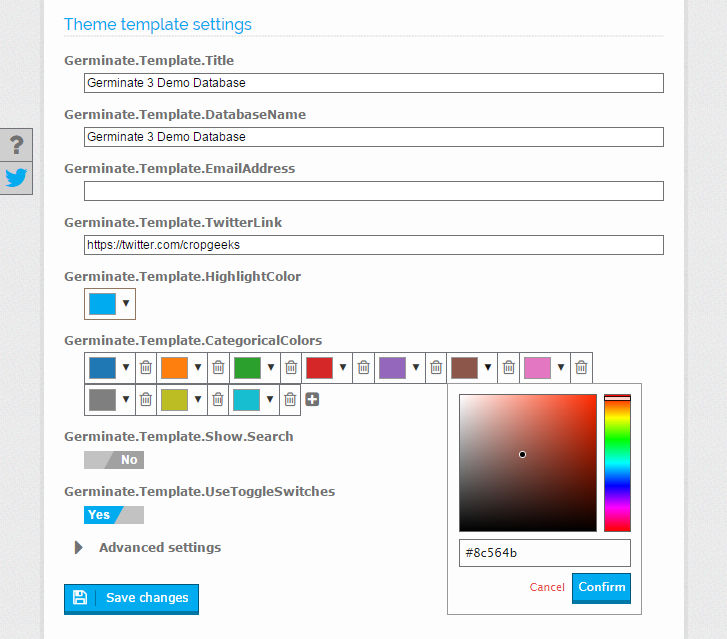
\includegraphics[scale=0.4]{img/configuration/admin-config.png}
	\caption{The Germinate configuration page available to administrators.}
	\label{fig:admin-config}
\end{figure}

\subsection{Germinate Menu}
\label{sec:menu}
Germinate uses a predefined menu structure by default. This default menu setup is based on what we think is a reasonable structure. However, even we are not infallible, so we decided to make the menu customizable.

We will now explain how you can define your own, custom menu structure and we will then give an example of how this can be used.

\subsubsection{Structure}
The menu of Germinate can be defined in XML format. We will explain this format using the example below:

\begin{lstlisting}[style=Xml]
<menu>
	<item key="home">
		<label key="en_GB">Home</label>
		<label key="de_DE">Home</label>
	</item>
	<item key="category.data">
		<label key="en_GB">Data</label>
		<label key="de_DE">Daten</label>
		<item key="browse-accessions">
			<label key="en_GB">Accessions</label>
			<label key="de_DE">Muster</label>
		</item>
		<item key="category.molecular">
			<label key="en_GB">Molecular data</label>
			<label key="de_DE">Molekulare Daten</label>
			<item key="genotype-datasets">
				<label key="en_GB">Genotypes</label>
				<label key="de_DE">Genotypen</label>
			</item>
			<item key="map-details">
				<label key="en_GB">Maps</label>
				<label key="de_DE">Molekulare Karten</label>
			</item>
		</item>
	</item>
	<item key="category.environment">
		<label key="en_GB">Environment</label>
		<label key="de_DE">Umwelt</label>
		<item key="geographic-search">
			<label key="en_GB">Geographic search</label>
			<label key="de_DE">Geografische Suche</label>
		</item>
	</item>
</menu>
\end{lstlisting}
\noindent
This will result in the following menu structure:\\
\\
\begin{tabular}[t]{@{}>{\raggedright\arraybackslash}p{0.5\textwidth}}
	\textbf{British English}:
	\begin{itemize}
		\item Home
		\item Data
		\begin{itemize}
			\item Accessions
			\item Molecular data
			\begin{itemize}
				\item Genotypes
				\item Maps
			\end{itemize}
		\end{itemize}
		\item Environment
		\begin{itemize}
			\item Geographic search	
		\end{itemize}
	\end{itemize}
\end{tabular}
\begin{tabular}[t]{@{}>{\raggedright\arraybackslash}p{0.5\textwidth}}
	\textbf{German}:
	\begin{itemize}
		\item Home
		\item Daten
		\begin{itemize}
			\item Muster
			\item Molekulare Daten
			\begin{itemize}
				\item Genotypen
				\item Genetische Karten
			\end{itemize}
		\end{itemize}
		\item Umwelt
		\begin{itemize}
			\item Geographische Suche
		\end{itemize}
	\end{itemize}
\end{tabular}
\noindent
We will now explain the individual elements of the XML file:
\begin{description}
	\item[\texttt{menu}] The root element of the XML file.
	\item[\texttt{item}] This is used for any menu element. This can either be a link to an actual page, or a submenu.
	\item[\texttt{item key}] If this item represents an actual Germinate Page (cf. Section \ref{sec:pages}) then this has to be the name of the page. If this item is a sub-menu, then this has to be a unique id.
	\item[\texttt{label}] Labels are used as the text content of the menu item, i.e. what the user will see. Every item has to provide this information for ALL of the supported languages (cf. Section \ref{sec:i18n}).
	\item[\texttt{label key}] The locale of the supported language.
\end{description}